\apendice{Especificación de Requisitos}
\section{Diagrama de casos de uso}


En la Figura~\ref{fig: casos de uso} se presenta el diagrama de casos de uso de la aplicación realizada, en el que se describen las distintas interacciones que pueden realizar los usuarios, dependiendo de si tienen MATLAB instalado o no.

\begin{itemize}
    \item El \textbf{usuario con MATLAB} puede abrir directamente la aplicación desde el archivo \texttt{.mlapp}, seleccionar el modelo epidemiológico, introducir los parámetros, ejecutar la simulación y visualizar los resultados, también se puede simular desdpués de elegir el modelo ya que .
    
    \item El \textbf{usuario sin MATLAB} debe primero instalar los \textit{MATLAB Runtimes} mediante el instalador \texttt{myAppInstaller\_web.exe}, y posteriormente ejecutar la aplicación compilada \texttt{.exe}. Una vez completados estos pasos, podrá seguir el mismo flujo funcional que el usuario con MATLAB.
    
    \item Los casos de uso principales compartidos por ambos tipos de usuario son: \textit{Seleccionar modelo}, \textit{Introducir parámetros}, \textit{Simular} y \textit{Visualización de resultados}.
\end{itemize}

\begin{figure}[H]
        \centering
        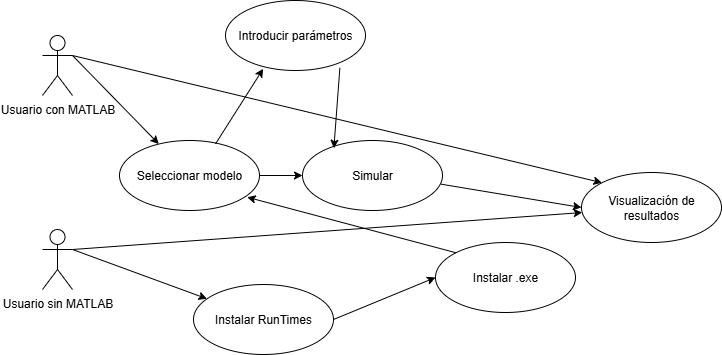
\includegraphics[width=0.9\textwidth]{img/diagrama casos.drawio.png}
        \caption{Diagrama de casos de uso de la aplicación realizada.}
        \label{fig: casos de uso}
        
\end{figure}


\section{Explicación casos de uso}
A continuación en las diferentes tablas (\ref{tab:cu1})(\ref{tab:cu2})(\ref{tab:cu3})(\ref{tab:cu4})(\ref{tab:cu5})(\ref{tab:cu6}) se detalla la explicación de los casos de usos utilizados en el diagraama de casos de uso del apartado anterior.
\begin{table}[H]
\centering
\begin{tabular}{|p{3cm}|p{9cm}|}
\hline
\textbf{CU-1} & \textbf{Seleccionar modelo} \\
\hline
\textbf{Versión} & 1.0 \\
\hline
\textbf{Autor} & Lucía Segura Benito \\
\hline
\textbf{Requisitos asociados} & RF-01 \\
\hline
\textbf{Descripción} & El usuario selecciona el tipo de modelo epidemiológico a utilizar: SI, SIS, SIR, SEIR, SIRV o SEIRV. \\
\hline
\textbf{Precondición} & La aplicación debe estar abierta. \\
\hline
\textbf{Acciones} &
\begin{enumerate}
    \item El usuario abre el menú desplegable de modelos.
    \item Selecciona uno de los modelos disponibles.
    \item El sistema guarda la selección para la simulación posterior.
\end{enumerate}
\\
\hline
\textbf{Postcondición} & Modelo seleccionado queda registrado en la aplicación. \\
\hline
\textbf{Excepciones} & No se produce ninguna si el desplegable está bien cargado. \\
\hline
\textbf{Importancia} & Alta \\
\hline
\end{tabular}
\caption{CU-1: Seleccionar modelo.}
\label{tab:cu1}
\end{table}



\begin{table}[H]
\centering
\begin{tabular}{|p{3cm}|p{9cm}|}
\hline
\textbf{CU-2} & \textbf{Introducir parámetros} \\
\hline
\textbf{Versión} & 1.0 \\
\hline
\textbf{Autor} & Lucía Segura Benito \\
\hline
\textbf{Requisitos asociados} & RF-02 \\
\hline
\textbf{Descripción} & El usuario introduce los valores numéricos requeridos para simular el modelo seleccionado. \\
\hline
\textbf{Precondición} & Un modelo debe estar previamente seleccionado. \\
\hline
\textbf{Acciones} &
\begin{enumerate}
    \item El usuario accede a los campos de parámetros.
    \item Introduce valores que se piden dependiendo del modelo seleccionado.
    \item El sistema almacena los parámetros para usarlos en la simulación.
\end{enumerate}
\\
\hline
\textbf{Postcondición} & Parámetros definidos correctamente para la simulación. \\
\hline
\textbf{Excepciones} & Parámetros vacíos o no válidos (el sistema muestra mensaje de error). \\
\hline
\textbf{Importancia} & Alta \\
\hline
\end{tabular}
\caption{CU-2: Introducir parámetros.}
\label{tab:cu2}
\end{table}






\begin{table}[H]
\centering
\begin{tabular}{|p{3cm}|p{9cm}|}
\hline
\textbf{CU-3} & \textbf{Simular modelo} \\
\hline
\textbf{Versión} & 1.0 \\
\hline
\textbf{Autor} & Lucía Segura Benito \\
\hline
\textbf{Requisitos asociados} & RF-03, RF-04 \\
\hline
\textbf{Descripción} & El usuario ejecuta la simulación del modelo epidemiológico seleccionado utilizando los parámetros introducidos. \\
\hline
\textbf{Precondición} & El modelo debe estar seleccionado y los parámetros correctamente definidos. \\
\hline
\textbf{Acciones} &
\begin{enumerate}
    \item El usuario pulsa el botón "Simular".
    \item El sistema verifica que los datos de entrada sean válidos.
    \item El sistema ejecuta el modelo epidemiológico seleccionado.
    \item Se muestran los resultados en pantalla mediante gráficas.
\end{enumerate}
\\
\hline
\textbf{Postcondición} & Los resultados de la simulación se visualizan en la interfaz de usuario. \\
\hline
\textbf{Excepciones} & Parámetros incompletos o inválidos (el sistema muestra un mensaje de error). \\
\hline
\textbf{Importancia} & Alta \\
\hline
\end{tabular}
\caption{CU-3: Simular modelo.}
\label{tab:cu3}
\end{table}



\begin{table}[H]
\centering
\begin{tabular}{|p{3cm}|p{9cm}|}
\hline
\textbf{CU-4} & \textbf{Visualización de resultados} \\
\hline
\textbf{Versión} & 1.0 \\
\hline
\textbf{Autor} & Lucía Segura Benito \\
\hline
\textbf{Requisitos asociados} & RF-05 \\
\hline
\textbf{Descripción} & La aplicación muestra al usuario los resultados de la simulación mediante gráficos. \\
\hline
\textbf{Precondición} & Simulación completada exitosamente. \\
\hline
\textbf{Acciones} &
\begin{enumerate}
    \item El sistema genera gráficos de las variables.
    \item Los gráficos se muestran en la interfaz.
\end{enumerate}
\\
\hline
\textbf{Postcondición} & Gráficas epidemiológicas visibles para el usuario. \\
\hline
\textbf{Excepciones} & Error al renderizar gráficos (muy raro). \\
\hline
\textbf{Importancia} & Media \\
\hline
\end{tabular}
\caption{CU-4: Visualización de resultados.}
\label{tab:cu4}
\end{table}




\begin{table}[H]
\centering
\begin{tabular}{|p{3cm}|p{9cm}|}
\hline
\textbf{CU-5} & \textbf{Instalar RunTimes} \\
\hline
\textbf{Versión} & 1.0 \\
\hline
\textbf{Autor} & Lucía Segura Benito \\
\hline
\textbf{Requisitos asociados} & RF-06 \\
\hline
\textbf{Descripción} & El usuario sin MATLAB instala los MATLAB Runtime necesarios para ejecutar la aplicación compilada. \\
\hline
\textbf{Precondición} & No disponer de MATLAB instalado. Tener el archivo \texttt{myAppInstaller\_web.exe}. \\
\hline
\textbf{Acciones} &
\begin{enumerate}
    \item El usuario ejecuta el archivo \texttt{myAppInstaller\_web.exe}.
    \item El instalador descarga e instala los runtimes de MATLAB (MCR).
\end{enumerate}
\\
\hline
\textbf{Postcondición} & Los runtimes de MATLAB quedan correctamente instalados. \\
\hline
\textbf{Excepciones} & Error en la instalación por permisos, red o espacio en disco. \\
\hline
\textbf{Importancia} & Alta \\
\hline
\end{tabular}
\caption{CU-5: Instalar RunTimes.}
\label{tab:cu5}
\end{table}




\begin{table}[H]
\centering
\begin{tabular}{|p{3cm}|p{9cm}|}
\hline
\textbf{CU-6} & \textbf{Instalar .exe} \\
\hline
\textbf{Versión} & 1.0 \\
\hline
\textbf{Autor} & Lucía Segura Benito \\
\hline
\textbf{Requisitos asociados} & RF-07 \\
\hline
\textbf{Descripción} & El usuario sin MATLAB ejecuta el archivo compilado de la aplicación tras instalar los runtimes. \\
\hline
\textbf{Precondición} & MATLAB Runtime (MCR) instalado previamente. \\
\hline
\textbf{Acciones} &
\begin{enumerate}
    \item El usuario ejecuta \texttt{aplicacion\_modelos.exe}.
    \item Se lanza la aplicación de forma autónoma, sin requerir MATLAB.
\end{enumerate}
\\
\hline
\textbf{Postcondición} & Aplicación ejecutándose de forma normal. \\
\hline
\textbf{Excepciones} & Error al lanzar el .exe, falta de runtimes o permisos insuficientes. \\
\hline
\textbf{Importancia} & Alta \\
\hline
\end{tabular}
\caption{CU-6: Instalar .exe.}
\label{tab:cu6}
\end{table}
